%% -*- mode: latex -*-
%% -*- mode: latex; -*-
%% \documentclass[conference]{IEEEtran}
\documentclass{article}

\input{header-common}

%% \include{pgfplots}

\usepackage[normalem]{ulem}

% I'm not terrifically happy with the available TODO packages...
% Alternatives are `todonotes` and `todo`
%% \usepackage{todonotes}
%% \presetkeys{todonotes}{inline}{}
%% \usepackage{siunitx}
%% \usepackage{todo}


\usepackage[scaled]{helvet}
\renewcommand\familydefault{\sfdefault}
\usepackage[top=2cm,bottom=2cm,outer=0.5in,inner=0.5in,landscape]{geometry}
\usepackage{multicol}
%% \usepackage[pages=some]{background}
%% \backgroundsetup{
%%   scale=0.5,
%%   %% color=black,
%%   %% opacity=0.5,
%%   angle=0,
%%   contents={
%%     \includegraphics[
%%       width=\pagewidth,
%%       height=\pageheight
%%     ]
%%                     {src/figures/map.eps}
%%   }
%% }

\pagestyle{empty}

\begin{document}
%% \begin{multicols}{2}
\twocolumn

\section*{SAGE Ski Trip 2015}
Hi!
We're glad you decided to come along for the 2015 SAGE Ski Trip to \textbf{Stowe Mountain Resort} from January 23--25.
We're staying at the \textbf{Commodore's Inn}, located at \emph{823 South Main Street, Stowe, VT 05672}.
Your primary point of contacts are \textbf{Zack Webster} \emph{(\missingdata)} and \textbf{Schuyler Eldridge} \emph{(\missingdata)}.

Our intended itinerary is as shown in Table \ref{tab-itinerary}.
Buses will leave Boston from the George Sherman Union (775 Commonwealth Ave) at 1745.
On our way to Stowe, we'll stop for fast food in West Lebanon, NH.
On both Saturday and Sunday, the buses will leave at 0730 and 0830 for Stowe Mountain Resort.
If you'd like to leave later, there is a free shuttle bus that stops at the Commodore's Inn every \todo{some amount of time}.
After the bus drops us off in the Mansfield Parking Lot, you'll have immediate access to skiing on Mount Mansfield.
For rentals, lessons, and easier skiing you can head to Spruce Peak using the \emph{Over Easy Transfer Gondola}.
Lessons begin at 1000 and 1330 \todo{check these times}.
The buses will pick us up from the resort at 1745 each day from the Mansfield Parking Lot.

Our hotel includes \textbf{breakfast from 0700--1030} and \textbf{dinner from 1730--2100}.
You're on your own for lunch, but the Spruce Peak lodge has an excellent cafeteria.
There will be a \textbf{SAGE Social} at the Commodore's Inn following dinner on Saturday.

As a new feature this year, we're trying to facilitate \emph{optional} ski groups if you'd like to ski with people of a similar level.
If you've never skied before, get in touch with \textbf{\missingdata} \emph{()} who will be around Lower Spruce Peak.
Beginners (comfortable on Green Circle terrain) can contact \textbf{()} and meet up at the Spruce Peak Lodge.
Intermediates (comfortable on Blue Square terrain) can contact \textbf{\missingdata} \emph{()} who will be around Mansfield.
Advanced skiers (comfortable on Black Diamond terrain) can contact \textbf{Schuyler Eldridge} \emph{(\missingdata)} who will be around Mansfield.

\begin{table}[h]
  \def\taw{0.14}
  \small
  \centering
  \caption{Itinerary}
  \label{tab-itinerary}
  \begin{tabular}{lll}
    \toprule
    Day & Time & Description\\
    \midrule
    \multirow{3}{*}{
      \begin{minipage}{\taw\columnwidth}
        Friday
      \end{minipage}}
    & 1700 & Board Bus at GSU\\
    & 2000 & Food Stop in West Lebanon, NH \\
    & 2100 & Arrive Commodore's Inn \\
    \midrule \multirow{5}{*}{
      \begin{minipage}{\taw\columnwidth}
        Saturday
        \end{minipage}}
    & 0730 & First Bus to Resort \\
    & 0830 & Second Bus to Resort \\
    & 1645 & Buses Return to Commodore's Inn \\
    & 1800 & Dinner \\
    & 2000 & SAGE Social \\
    \midrule \multirow{3}{*}{
      \begin{minipage}{\taw\columnwidth}
        Sunday
    \end{minipage}}
    & 0730 & First Bus to Resort \\
    & 0830 & Second Bus to Resort \\
    & 1645 & Buses Depart for Boston \\
    \bottomrule
  \end{tabular}
\end{table}

\begin{figure}
  \centering
  \begin{tikzpicture}
    % draw image
    \node[inner sep=0] at (current page.center)
         {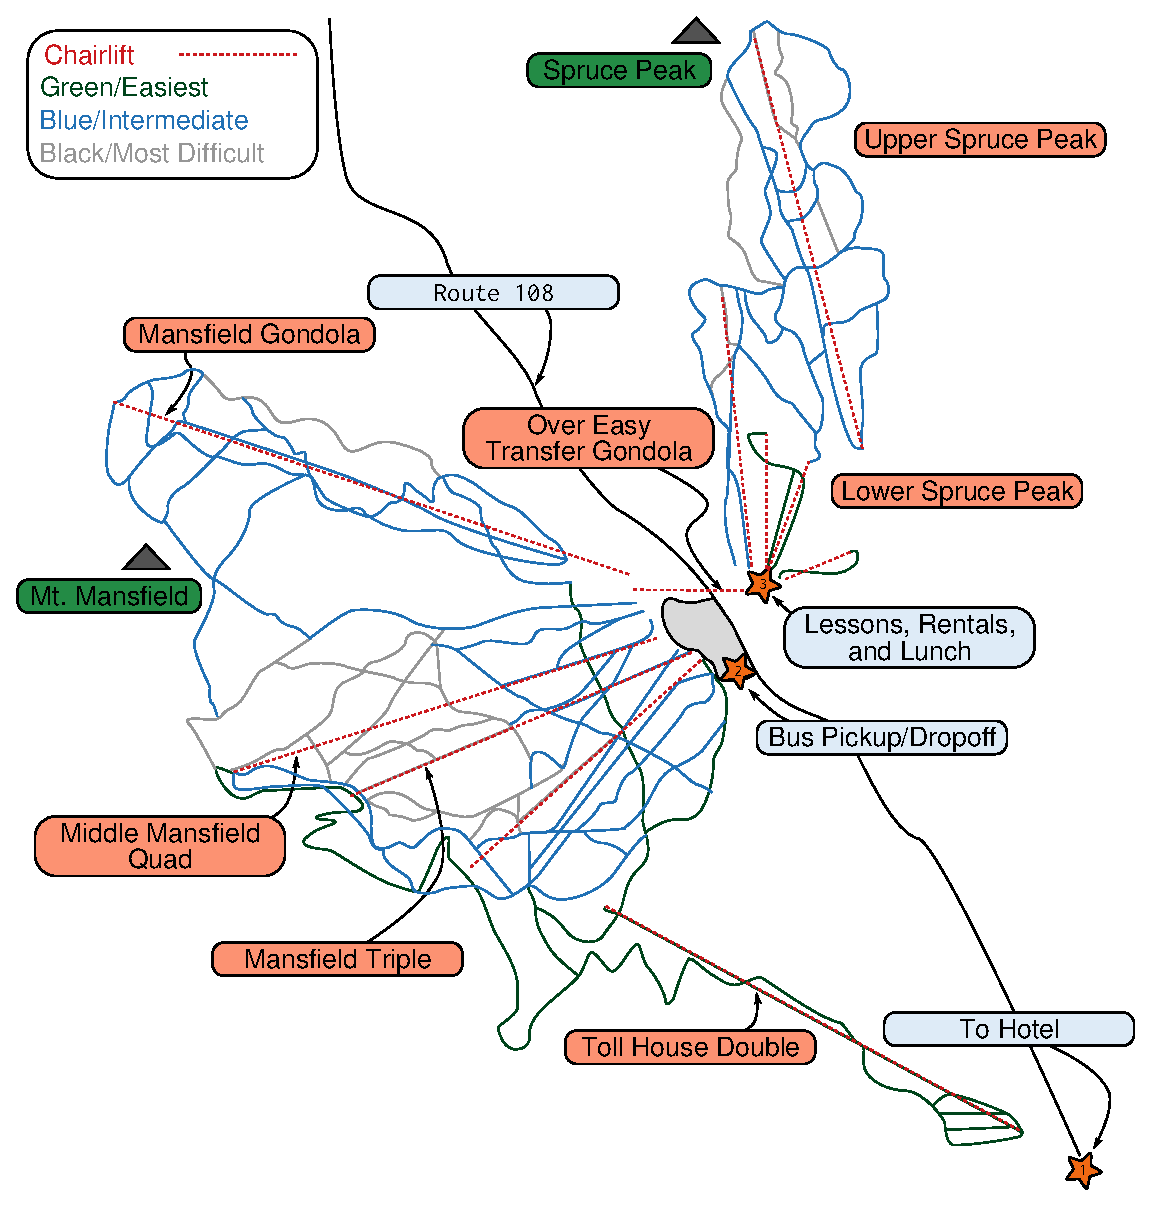
\includegraphics[width=0.9\columnwidth]{src/figures/map.eps}};
  \end{tikzpicture}
  \caption{Stowe Mountain Resort comprises two mountains, Mount Mansfield (serviced, primarily, by the \emph{Toll House Double}, \emph{Mansfield Triple}, \emph{Middle Mansfield Quad}, and \emph{Mansfield Gondola}) to the West and Spruce Peak (divided into Lower and Upper Spruce Peak) to the East.
    The \emph{Toll House Double} and \emph{Lower Spruce Peak} provide access to the easiest terrain, while all other areas and lifts have primarily intermediate and expert skiing.
    Mount Mansfield and Spruce Peak are divided by Route 108.
    You can move between them by using the \emph{Over Easy Transfer Gondola}.
    Lessons, rentals, and the main dining area are located at \emph{Lower Spruce Peak}, (3) on the map.
    Our hotel, the Commodore's Inn is located on Route 108, to the South, in the general direction of (1).
    In the morning and evening, our buses will drop off and pick up in the Mansfield parking lot at location (2).
  }
\end{figure}

%% \end{multicols}

\end{document}
